%% sections/02_motivation.tex

\section{동기: 왜 워크로드 레벨 게이팅이 필요한가}
\label{sec:motivation}

본 절은 \algname 의 두 설계 결정---워크로드 레벨 게이팅과 CPU 슬랙 하베스팅---이
왜 필요한지를 측정 데이터로 정당화한다.

%% -------------------------------------------------------------------------
\subsection{투기적 디코딩의 강력한 효과}
\label{subsec:mot-spec-power}

SuffixDecoding~\cite{snowflake-arctic} 기반 Trident core
(SuffixDecoding $+$ cudagraph PIECEWISE $+$ \texttt{gmu=0.80})는
H100 $\times$ 8 환경의 Llama-3.3-70B 모델에서 다음과 같은 처리량 향상을 달성한다.

%% figures/fig2_throughput_gain.tex
%% Fig.2 — Llama-3.3-70B 워크로드별 처리량 (vanilla / Trident / AGSD), 1컬럼

\begin{figure}[t]
\centering
\resizebox{0.95\columnwidth}{!}{%
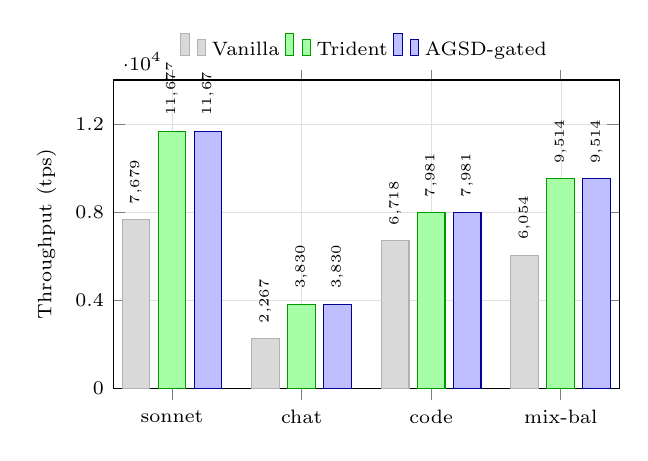
\begin{tikzpicture}
\begin{axis}[
    ybar=3pt,
    bar width=10pt,
    width=8cm, height=5.5cm,
    ylabel={Throughput (tps)},
    ylabel style={font=\scriptsize},
    symbolic x coords={sonnet, chat, code, mix-bal},
    xtick=data,
    xticklabel style={font=\scriptsize},
    yticklabel style={font=\scriptsize},
    ymin=0, ymax=14000,
    ytick={0,4000,8000,12000},
    legend style={at={(0.5,1.03)}, anchor=south, legend columns=3,
                  font=\scriptsize, draw=none},
    nodes near coords,
    nodes near coords style={font=\tiny, rotate=90, anchor=west, xshift=2pt},
    enlarge x limits=0.15,
    grid=major,
    grid style={line width=0.1pt, draw=gray!25},
]
\addplot[fill=gray!30, draw=gray!60] coordinates {
    (sonnet,7679) (chat,2267) (code,6718) (mix-bal,6054)};
\addplot[fill=green!35, draw=green!60!black] coordinates {
    (sonnet,11677) (chat,3830) (code,7981) (mix-bal,9514)};
\addplot[fill=blue!25, draw=blue!60!black] coordinates {
    (sonnet,11677) (chat,3830) (code,7981) (mix-bal,9514)};
\legend{Vanilla, Trident, AGSD-gated}
\end{axis}
\end{tikzpicture}%
}
\caption{Llama-3.3-70B + TP=8 + H100$\times$8 처리량 비교.
  Trident core가 모든 워크로드에서 vanilla 대비 $+18.8\%$--$+68.9\%$를 달성한다.
  Llama-70B는 전 워크로드에서 suffix가 최적이므로 AGSD $\equiv$ Trident.}
\label{fig:throughput-gain}
\end{figure}


\begin{table}[t]
\centering
\caption{Trident core vs.\ vanilla: Llama-3.3-70B, TP=8, H100$\times$8,
  500 prompts $\times$ 8192 max tokens (SUB\_093).}
\label{tbl:trident-vs-vanilla}
\footnotesize
\begin{tabular}{@{}lrrl@{}}
\toprule
\textbf{Workload} & \textbf{Vanilla (tps)} & \textbf{Trident (tps)} & \textbf{$\Delta$} \\
\midrule
sonnet  & 7,678.7  & 11,676.9 & $\mathbf{+52.1\%}$ \\
chat    & 2,266.8  & 3,830.4  & $\mathbf{+68.9\%}$ \\
code    & 6,717.7  & 7,981.4  & $\mathbf{+18.8\%}$ \\
mix-sh  & 6,325.9  & 10,297.7 & $+62.8\%$ \\
mix-bal & 6,053.9  & 9,514.3  & $+57.2\%$ \\
mix-ch  & 6,494.9  & 9,457.3  & $+45.6\%$ \\
\bottomrule
\end{tabular}
\end{table}

Table~\ref{tbl:trident-vs-vanilla}이 보여주듯, 투기적 디코딩은 6개 워크로드
전체에서 순 양성(net positive)이며 처리량 향상은 $+18.8\%$에서 $+68.9\%$에 달한다.
그러나 워크로드 간 효과 편차가 3.7배에 이른다는 사실에 주목해야 한다.
code 워크로드의 이득($+18.8\%$)은 chat($+68.9\%$)의 약 $\frac{1}{4}$에 불과하다.
이 편차의 근본 원인을 다음 절에서 분석한다.

%% -------------------------------------------------------------------------
\subsection{Code Workload에서의 구조적 실패}
\label{subsec:mot-code-fail}

투기적 디코딩의 순이익은 R/K 비율로 결정된다
(\S\ref{subsec:rk-framework}).

\begin{equation}
\text{net gain} \propto \frac{K}{R} - 1, \quad K > R \Rightarrow \text{gain},
\quad K < R \Rightarrow \text{regression}
\label{eq:rk-condition}
\end{equation}

n-gram 드래프터의 code 워크로드에서 accept rate $\alpha$가 극도로 낮다.

\begin{table}[t]
\centering
\caption{드래프터별 $\alpha$와 $K$ 비교 (Llama-3.3-70B, SUB\_093).}
\label{tbl:alpha-k}
\footnotesize
\begin{tabular}{@{}llrrrr@{}}
\toprule
\textbf{Workload} & \textbf{Method} & $\boldsymbol{\alpha}$ & $\boldsymbol{K}$ & \textbf{$\Delta$ tps} \\
\midrule
code & ngram   & $1.2\%$  & $1.09$ & $\mathbf{-20.2\%}$ \\
code & suffix  & $40.1\%$ & $4.08$ & $+18.8\%$ \\
\midrule
sonnet & ngram  & $9.5\%$  & $1.66$ & $+40.1\%$ \\
sonnet & suffix & $77.0\%$ & $5.11$ & $+52.1\%$ \\
\midrule
chat   & ngram  & $71.2\%$ & $5.98$ & $+43.1\%$ \\
chat   & suffix & $92.7\%$ & $10.06$ & $+68.9\%$ \\
\bottomrule
\end{tabular}
\end{table}

Table~\ref{tbl:alpha-k}에서 n-gram 드래프터의 code $\alpha = 1.2\%$는
sonnet($9.5\%$) 대비 $8\times$ 낮으며, 이로 인해 $K = 1.09 < R$이 되어
$-20.2\%$의 catastrophic regression이 발생한다.
n-gram 드래프터는 입력 프롬프트 내 n-gram 패턴만을 활용하기 때문에,
자연어 텍스트와 달리 고유한 식별자와 키워드로 구성된 코드의
비반복적 토큰 분포에서 매우 낮은 hit rate를 보인다.

\textbf{Code agent에서의 심화.}
최근 급부상하는 code agent 응용---도구 호출(tool calling),
추론 체인(reasoning chain), 코드 디버깅 루프---에서는 이 문제가 더욱 심각하다.
Code agent는 동일 세션 내에서 LLM을 수십~수백 회 반복 호출하며,
각 호출마다 투기적 디코딩 스텝 오버헤드가 누적된다.
$K < R$ 조건에서 다중 호출이 이루어지면 총 지연이 선형 이상으로 증가한다.

% TODO: code agent 패턴(tool calling, multi-turn) 특화 측정 실험 추가.
%       현재 실험 setup(500 prompts × max_tokens=32)에서
%       code agent 시뮬레이션(n_turns=10, tool_call_ratio=0.5) 별도 SUB 필요.

%% -------------------------------------------------------------------------
\subsection{Suffix가 Code를 구제하지만 완전하지 않다}
\label{subsec:mot-suffix-limit}

SuffixDecoding~\cite{snowflake-arctic}은 입력 프롬프트뿐 아니라
이전 생성 출력까지 suffix tree에 누적하여 드래프팅에 활용한다.
이를 통해 code 워크로드에서 $\alpha$를 $1.2\% \to 40.1\%$로
($33\times$) 끌어올리고 $K = 4.08$을 달성하여 $+18.8\%$의 순 양성을 확보한다.

그러나 suffix 방법도 모든 환경에서 최적이 아니다.

\begin{table}[t]
\centering
\caption{모델 아키텍처별 code 워크로드 suffix 효과 (SUB\_096).}
\label{tbl:suffix-code-arch}
\footnotesize
\begin{tabular}{@{}lrrr@{}}
\toprule
\textbf{Model}       & \textbf{Vanilla} & \textbf{Suffix} & \textbf{$\Delta$} \\
\midrule
Llama-3.3-70B        & 6,717.7 & 7,981.4 & $+18.8\%$ \\
Phi-3-medium-14B     & 3,340   & 5,085   & $+52.2\%$ \\
\textbf{Qwen-2.5-72B}& \textbf{6,227}  & \textbf{5,941}  & $\mathbf{-5.0\%}$ \\
\bottomrule
\end{tabular}
\end{table}

Table~\ref{tbl:suffix-code-arch}에서 Qwen-2.5-72B의 code 워크로드에서
suffix가 $-5\%$ 회귀를 보인다.
이는 모델 아키텍처가 suffix tree의 패턴 적합성에 영향을 미침을 의미하며,
단일 투기적 디코딩 설정으로 모든 모델·워크로드 조합을 최적화하는 것이
원리적으로 불가능함을 보여준다.

% TODO: Qwen-2.5-72B code 워크로드에서 suffix 회귀의 메커니즘 분석.
%       tokenizer vocabulary 분포 차이, attention pattern 분포 측정 추가.

\textbf{결론.}
같은 서버에 sonnet($+52\%$)과 code agent($K < R$ 가능)가 혼재하는 운영 환경에서
단일 투기적 디코딩 설정은 구조적으로 최적화 불가능하다.
요청별(per-request) 방법 선택, 즉 \emph{워크로드 레벨 게이팅}이 필수적이다.

%% -------------------------------------------------------------------------
\subsection{기존 접근: llm-d의 복잡성}
\label{subsec:mot-llmd}

워크로드 인지 라우팅 문제를 해결하기 위한 대표적 접근으로
llm-d~\cite{llmd2025}가 있다.
llm-d는 Kubernetes 기반의 LLM disaggregation 프레임워크로,
prefill과 decode 단계를 분리된 노드로 분산하고
워크로드 특성에 따라 요청을 라우팅하는 정교한 구조를 채택한다.

% TODO: llm-d vs CERES 배포 복잡도 정량 비교 (컴포넌트 수, 설정 파라미터 수,
%       배포 시간, 운영 복잡도 지표).
%       현재 llm-d 공개 문서 기반 분석만 가능; 실제 배포 실험은 future work.

llm-d의 접근은 강력하지만 다음 한계가 있다.
(1) Kubernetes 클러스터 관리, 노드 간 KV 캐시 전송, 스케줄러 커스터마이징 등
복잡한 인프라 요구사항이 수반된다.
(2) 단일 서버 수준에서의 경량 배포에는 적합하지 않다.
(3) 투기적 디코딩의 워크로드별 최적 방법 선택을
핵심 설계 목표로 다루지 않는다.

\algname 은 이와 달리 기존 vLLM 스택에 \emph{최소 침습적(minimally invasive)} 변경만으로
워크로드 레벨 게이팅을 구현한다:
외부 분류기는 FastAPI + ProcessPool 기반 경량 프로세스,
백엔드 라우팅은 HTTP 포워딩이며 vLLM 코어 변경은 14줄에 불과하다.

%% -------------------------------------------------------------------------
\subsection{게이팅이 CPU 슬랙을 낳는다}
\label{subsec:mot-cpu-slack}

워크로드 레벨 게이팅을 구현하면 두 개의 vLLM 인스턴스를 병렬 운영하는
이중 백엔드 구조가 자연스럽게 발생한다.
이 구조는 CPU 유휴를 \emph{필연적}으로 생성한다.

\begin{itemize}
\item 두 인스턴스가 각자 별도 GPU 그룹을 점유하므로
  (GPU 0--3: vanilla backend, GPU 4--7: Trident backend),
  NUMA 노드도 GPU PCIe affinity에 따라 자연 분리된다.
\item 각 인스턴스의 CPU 이용률은 Trident $5.3\%$, vanilla $5.6\%$로
  $94\%$ 이상의 CPU가 유휴 상태다 (SUB\_093 config-wide 평균).
\item 듀얼-NUMA 아키텍처에서 remote/local 접근 거리 비가 $2.1\times$이므로
  NUMA 비인지(NUMA-unaware) 배치는 지속적인 지연 패널티를 초래한다.
\end{itemize}

이 CPU 유휴는 \algname 의 두 번째 구성요소인 \emph{CPU 슬랙 하베스팅}의
재료가 된다.
NUMA 바인딩으로 cross-socket QPI 트래픽을 제거하고,
스텝 경계 정렬 branchy 보조 작업으로 유휴 CPU 사이클을 수확한다
(\S\ref{sec:ceres}).

\textbf{요약.}
투기적 디코딩은 강력하지만 워크로드 의존적이고, code workload에서 구조적 위험이 있으며,
이를 해결하면 CPU 슬랙이 생긴다.
\algname 은 이 두 문제를 연결된 하나의 구조로 해결한다.
